\documentclass{standalone}
\usepackage{tikz}
\usetikzlibrary{patterns, positioning}


\begin{document}
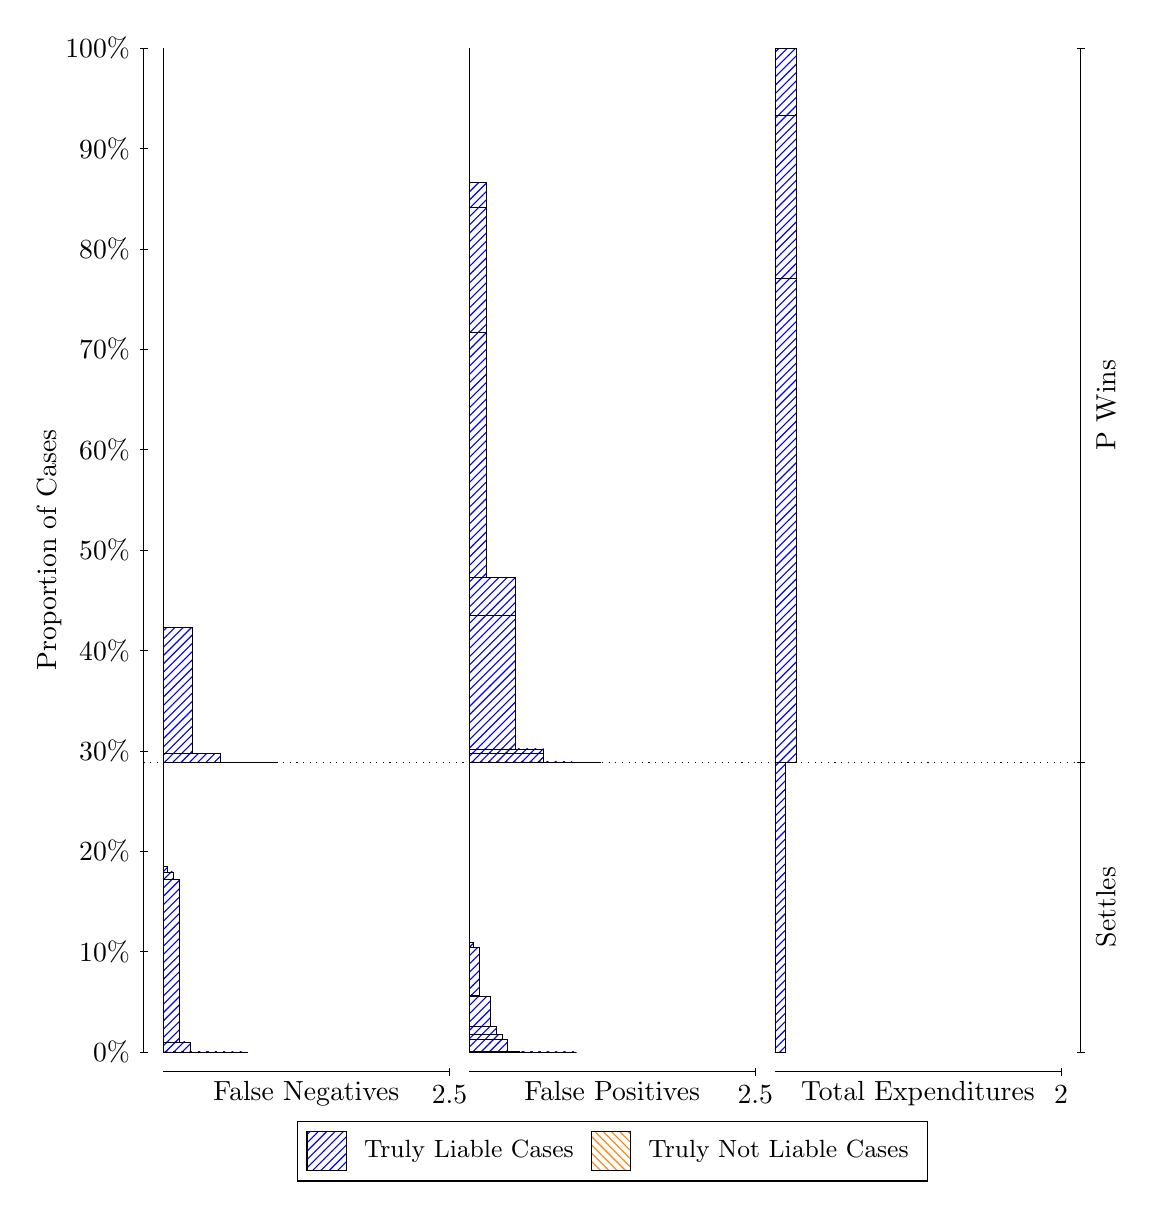
\begin{tikzpicture}
\draw[black, very thin] (1.5,1.75) -- (1.5,14.5);
\node[rotate=90, text=black, anchor=center] at (0.3, 8.125) {Proportion of Cases};
\draw[black, very thin] (1.45,1.75) -- (1.55,1.75);
\node[text=black, anchor=east] at (1.45, 1.75) {0\%};
\draw[black, very thin] (1.45,3.025) -- (1.55,3.025);
\node[text=black, anchor=east] at (1.45, 3.025) {10\%};
\draw[black, very thin] (1.45,4.3) -- (1.55,4.3);
\node[text=black, anchor=east] at (1.45, 4.3) {20\%};
\draw[black, very thin] (1.45,5.575) -- (1.55,5.575);
\node[text=black, anchor=east] at (1.45, 5.575) {30\%};
\draw[black, very thin] (1.45,6.85) -- (1.55,6.85);
\node[text=black, anchor=east] at (1.45, 6.85) {40\%};
\draw[black, very thin] (1.45,8.125) -- (1.55,8.125);
\node[text=black, anchor=east] at (1.45, 8.125) {50\%};
\draw[black, very thin] (1.45,9.4) -- (1.55,9.4);
\node[text=black, anchor=east] at (1.45, 9.4) {60\%};
\draw[black, very thin] (1.45,10.675) -- (1.55,10.675);
\node[text=black, anchor=east] at (1.45, 10.675) {70\%};
\draw[black, very thin] (1.45,11.95) -- (1.55,11.95);
\node[text=black, anchor=east] at (1.45, 11.95) {80\%};
\draw[black, very thin] (1.45,13.225) -- (1.55,13.225);
\node[text=black, anchor=east] at (1.45, 13.225) {90\%};
\draw[black, very thin] (1.45,14.5) -- (1.55,14.5);
\node[text=black, anchor=east] at (1.45, 14.5) {100\%};

\draw[black, very thin] (13.4,1.75) -- (13.4,14.5);
\draw[black, very thin] (13.35,1.75) -- (13.45,1.75);
\node[anchor=west] at (13.35, 1.75) {};
\draw[black, very thin] (13.35,5.4314) -- (13.45,5.4314);
\node[anchor=west] at (13.35, 5.4314) {};
\draw[black, very thin] (13.35,14.5) -- (13.45,14.5);
\node[anchor=west] at (13.35, 14.5) {};

\draw[black, very thin, pattern color=blue, pattern=north east lines] (1.75,1.75) rectangle (2.8218,1.75);
\draw[black, very thin, pattern color=blue, pattern=north east lines] (1.75,1.75) rectangle (2.5312,1.75);
\draw[black, very thin, pattern color=blue, pattern=north east lines] (1.75,1.75) rectangle (2.4585,1.7506);
\draw[black, very thin, pattern color=blue, pattern=north east lines] (1.75,1.7506) rectangle (2.3858,1.7506);
\draw[black, very thin, pattern color=blue, pattern=north east lines] (1.75,1.7506) rectangle (2.2405,1.7508);
\draw[black, very thin, pattern color=blue, pattern=north east lines] (1.75,1.7508) rectangle (2.1678,1.7517);
\draw[black, very thin, pattern color=blue, pattern=north east lines] (1.75,1.7517) rectangle (2.0952,1.8756);
\draw[black, very thin, pattern color=blue, pattern=north east lines] (1.75,1.8756) rectangle (2.0952,1.8767);
\draw[black, very thin, pattern color=blue, pattern=north east lines] (1.75,1.8767) rectangle (2.0225,1.8769);
\draw[black, very thin, pattern color=blue, pattern=north east lines] (1.75,1.8769) rectangle (1.9498,3.9449);
\draw[black, very thin, pattern color=blue, pattern=north east lines] (1.75,3.9449) rectangle (1.8772,4.0369);
\draw[black, very thin, pattern color=blue, pattern=north east lines] (1.75,4.0369) rectangle (1.8045,4.1041);
\draw[black, very thin, pattern color=orange, pattern=north west lines] (1.75,4.1041) rectangle (1.75,4.1041);
\draw[black, very thin, pattern color=blue, pattern=north east lines] (1.75,4.1041) rectangle (1.75,5.4314);
\draw[black, very thin, pattern color=blue, pattern=north east lines] (1.75,5.4314) rectangle (3.2033,5.4314);
\draw[black, very thin, pattern color=blue, pattern=north east lines] (1.75,5.4314) rectangle (2.84,5.4326);
\draw[black, very thin, pattern color=blue, pattern=north east lines] (1.75,5.4326) rectangle (2.4767,5.5442);
\draw[black, very thin, pattern color=blue, pattern=north east lines] (1.75,5.5442) rectangle (2.1133,7.1376);
\draw[black, very thin, pattern color=orange, pattern=north west lines] (1.75,7.1376) rectangle (1.75,7.1376);
\draw[black, very thin, pattern color=blue, pattern=north east lines] (1.75,7.1376) rectangle (1.75,14.5);
\draw[black, very thin, pattern color=orange, pattern=north west lines] (5.6333,1.75) rectangle (6.9958,1.75);
\draw[black, very thin, pattern color=blue, pattern=north east lines] (5.6333,1.75) rectangle (6.9958,1.75);
\draw[black, very thin, pattern color=orange, pattern=north west lines] (5.6333,1.75) rectangle (6.8505,1.75);
\draw[black, very thin, pattern color=blue, pattern=north east lines] (5.6333,1.75) rectangle (6.8505,1.75);
\draw[black, very thin, pattern color=orange, pattern=north west lines] (5.6333,1.75) rectangle (6.7052,1.75);
\draw[black, very thin, pattern color=blue, pattern=north east lines] (5.6333,1.75) rectangle (6.7052,1.75);
\draw[black, very thin, pattern color=blue, pattern=north east lines] (5.6333,1.75) rectangle (6.6325,1.75);
\draw[black, very thin, pattern color=orange, pattern=north west lines] (5.6333,1.75) rectangle (6.5598,1.75);
\draw[black, very thin, pattern color=blue, pattern=north east lines] (5.6333,1.75) rectangle (6.5598,1.75);
\draw[black, very thin, pattern color=blue, pattern=north east lines] (5.6333,1.75) rectangle (6.4872,1.75);
\draw[black, very thin, pattern color=orange, pattern=north west lines] (5.6333,1.75) rectangle (6.4145,1.75);
\draw[black, very thin, pattern color=blue, pattern=north east lines] (5.6333,1.75) rectangle (6.4145,1.7507);
\draw[black, very thin, pattern color=blue, pattern=north east lines] (5.6333,1.7507) rectangle (6.3418,1.7513);
\draw[black, very thin, pattern color=blue, pattern=north east lines] (5.6333,1.7513) rectangle (6.2692,1.7536);
\draw[black, very thin, pattern color=blue, pattern=north east lines] (5.6333,1.7536) rectangle (6.1965,1.7536);
\draw[black, very thin, pattern color=blue, pattern=north east lines] (5.6333,1.7536) rectangle (6.1238,1.7545);
\draw[black, very thin, pattern color=orange, pattern=north west lines] (5.6333,1.7545) rectangle (6.1238,1.7545);
\draw[black, very thin, pattern color=blue, pattern=north east lines] (5.6333,1.7545) rectangle (6.1238,1.9146);
\draw[black, very thin, pattern color=blue, pattern=north east lines] (5.6333,1.9146) rectangle (6.0512,1.9718);
\draw[black, very thin, pattern color=blue, pattern=north east lines] (5.6333,1.9718) rectangle (5.9785,2.0738);
\draw[black, very thin, pattern color=blue, pattern=north east lines] (5.6333,2.0738) rectangle (5.9058,2.454);
\draw[black, very thin, pattern color=blue, pattern=north east lines] (5.6333,2.454) rectangle (5.8332,2.4542);
\draw[black, very thin, pattern color=blue, pattern=north east lines] (5.6333,2.4542) rectangle (5.7605,2.4754);
\draw[black, very thin, pattern color=blue, pattern=north east lines] (5.6333,2.4754) rectangle (5.7605,3.0773);
\draw[black, very thin, pattern color=blue, pattern=north east lines] (5.6333,3.0773) rectangle (5.6878,3.1445);
\draw[black, very thin, pattern color=blue, pattern=north east lines] (5.6333,3.1445) rectangle (5.6333,5.4314);
\draw[black, very thin, pattern color=orange, pattern=north west lines] (5.6333,5.4314) rectangle (7.3047,5.4314);
\draw[black, very thin, pattern color=blue, pattern=north east lines] (5.6333,5.4314) rectangle (7.3047,5.4314);
\draw[black, very thin, pattern color=orange, pattern=north west lines] (5.6333,5.4314) rectangle (6.9413,5.4314);
\draw[black, very thin, pattern color=blue, pattern=north east lines] (5.6333,5.4314) rectangle (6.9413,5.4328);
\draw[black, very thin, pattern color=blue, pattern=north east lines] (5.6333,5.4328) rectangle (6.9413,5.4336);
\draw[black, very thin, pattern color=orange, pattern=north west lines] (5.6333,5.4336) rectangle (6.578,5.4336);
\draw[black, very thin, pattern color=blue, pattern=north east lines] (5.6333,5.4336) rectangle (6.578,5.5481);
\draw[black, very thin, pattern color=blue, pattern=north east lines] (5.6333,5.5481) rectangle (6.578,5.5985);
\draw[black, very thin, pattern color=orange, pattern=north west lines] (5.6333,5.5985) rectangle (6.2147,5.5985);
\draw[black, very thin, pattern color=blue, pattern=north east lines] (5.6333,5.5985) rectangle (6.2147,7.2954);
\draw[black, very thin, pattern color=blue, pattern=north east lines] (5.6333,7.2954) rectangle (6.2147,7.7785);
\draw[black, very thin, pattern color=blue, pattern=north east lines] (5.6333,7.7785) rectangle (5.8513,10.893);
\draw[black, very thin, pattern color=orange, pattern=north west lines] (5.6333,10.893) rectangle (5.8513,10.893);
\draw[black, very thin, pattern color=blue, pattern=north east lines] (5.6333,10.893) rectangle (5.8513,12.476);
\draw[black, very thin, pattern color=blue, pattern=north east lines] (5.6333,12.476) rectangle (5.8513,12.794);
\draw[black, very thin, pattern color=blue, pattern=north east lines] (5.6333,12.794) rectangle (5.6333,14.5);
\draw[black, very thin, pattern color=orange, pattern=north west lines] (9.5167,1.75) rectangle (9.6529,1.75);
\draw[black, very thin, pattern color=blue, pattern=north east lines] (9.5167,1.75) rectangle (9.6529,5.4314);
\draw[black, very thin, pattern color=orange, pattern=north west lines] (9.5167,5.4314) rectangle (9.7892,5.4314);
\draw[black, very thin, pattern color=blue, pattern=north east lines] (9.5167,5.4314) rectangle (9.7892,11.57);
\draw[black, very thin, pattern color=orange, pattern=north west lines] (9.5167,11.57) rectangle (9.7892,11.57);
\draw[black, very thin, pattern color=blue, pattern=north east lines] (9.5167,11.57) rectangle (9.7892,13.647);
\draw[black, very thin, pattern color=orange, pattern=north west lines] (9.5167,13.647) rectangle (9.7892,13.647);
\draw[black, very thin, pattern color=blue, pattern=north east lines] (9.5167,13.647) rectangle (9.7892,14.5);
\draw[black, dotted] (1.5,5.4314) -- (13.4,5.4314);
\draw[black, very thin] (1.75,1.5) -- (5.3833,1.5);
\node[text=black, anchor=north] at (3.5667, 1.5) {False Negatives};
\draw[black, very thin] (5.3833,1.45) -- (5.3833,1.55);
\node[text=black, anchor=north] at (5.3833, 1.45) {2.5};

\draw[black, very thin] (5.6333,1.5) -- (9.2667,1.5);
\node[text=black, anchor=north] at (7.45, 1.5) {False Positives};
\draw[black, very thin] (9.2667,1.45) -- (9.2667,1.55);
\node[text=black, anchor=north] at (9.2667, 1.45) {2.5};

\draw[black, very thin] (9.5167,1.5) -- (13.15,1.5);
\node[text=black, anchor=north] at (11.333, 1.5) {Total Expenditures};
\draw[black, very thin] (13.15,1.45) -- (13.15,1.55);
\node[text=black, anchor=north] at (13.15, 1.45) {2};

\node[text=black, centered, rotate=90] at (13.72, 3.5907) {Settles};
\node[text=black, centered, rotate=90] at (13.72, 9.9657) {P Wins};

\draw (7.449999999999999,1.5) node[draw=none] (baseCoordinate) {};
\begin{scope}[align=center]
        \matrix[scale=0.5, draw=black, below=0.5cm of baseCoordinate, nodes={draw}, column sep=0.1cm]{
            \node[rectangle, draw, minimum width=0.5cm, minimum height=0.5cm, pattern color=blue, pattern=north east lines] {}; &
            \node[draw=none, font=\small, text=black] (B) {Truly Liable Cases}; &
            \node[rectangle, draw, minimum width=0.5cm, minimum height=0.5cm, pattern color=orange, pattern=north west lines] {}; &
            \node[draw=none, font=\small, text=black] (B) {Truly Not Liable Cases}; \\
            };
\end{scope}

\end{tikzpicture}
\end{document}